\ItemCategory{}
\ItemSubCategory{}
\ItemFolder{}

\chapter*{Bow of Growth}\stepcounter{section}\phantomsection\addcontentsline{toc}{section}{Bow of Growth}
\itemDescriptionAndImage{Wondrous Bow, Artifact (requires attunement by a Class-Lvl 3+ Ranger or Arcane Archer)}{images/Magic_Items/Bow_of_Growth.png}{6cm}\\

\begin{tikzpicture}[remember picture, overlay]%
	\node[xshift=0.7\columnwidth, yshift=-0.375\paperheight, rotate=-60] at (current page.center) {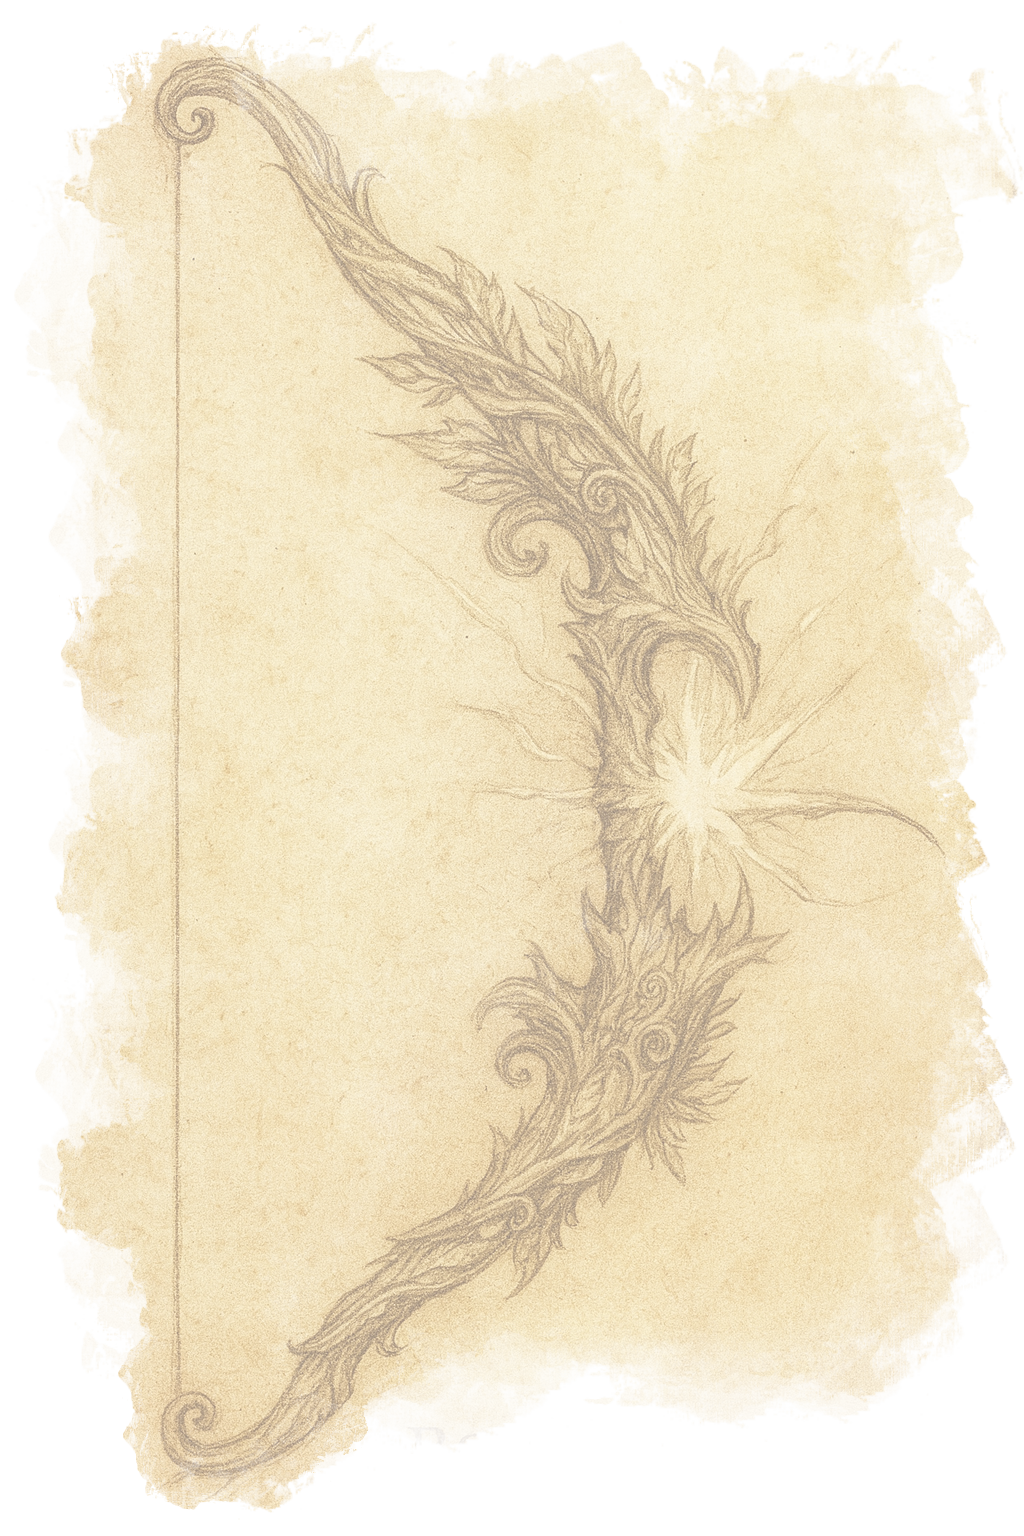
\includegraphics[width=0.9\columnwidth]{%
		images/Magic_Items/Bow_of_Growth_background.png%
	}};%
\end{tikzpicture}%

\section*{Appearance}
{\entryfont The Bow of Growth is an artifact that seems less crafted and more grown into existence. Its body is formed from ancient, living wood, dark and rich in color, with the texture of aged bark still visible along its surface. The limbs are curved with an almost organic elegance, twisting in patterns reminiscent of climbing vines. Intricate whorls and spirals are etched naturally into the wood, as if inscribed by time itself.

From the bow's frame sprout delicate leaf-like extensions, some vibrant green as though freshly budded, others appearing petrified like eternal foliage frozen in time. These leaves shift subtly in the light, glowing faintly with a verdant aura, hinting at the living magic coursing through the artifact.

At its heart, near the grip, the bow radiates a soft green luminescence, pulsing like the heartbeat of an ancient forest. Tiny motes of light drift lazily around it, evoking spores, pollen, or fireflies in the twilight. The string, fine and taut, appears spun from woven strands of golden sunlight and verdant magic, shimmering faintly as if it were never meant for mortal hands to pull.}
\section*{History}
{\entryfont Among the oldest tales of the elven tribes and ancient hunter lodges, the Bow of Growth is spoken of in hushed reverence. Legends say the bow is not forged, but summoned by the will of the wild itself. It is said to appear only after great calamities - when forests are cut down in vast numbers or when wildfires consume the green heart of the world. In such dark times, the bow emerges from roots and branches entwining themselves into its form, a gift of renewal from the spirits of the wood.

Those rare few who have wielded it claim the bow bears the power to strike down beasts no mortal weapon could touch - even creatures of the Feywild fall to its arrows. Yet more than a hunter's tool, it is a reminder: that nature will always regrow, and that even in ruin, life returns stronger than before.}
\vfill\eject
\section*{Magic}
{\entryfont The Bow of Growth is imbued with the raw, untamed power of nature itself. Arrows loosed from its string carry more than simple force - they strike with the will of the wild. Upon impact, thorny vines burst forth, entangling and piercing the struck foe, while the fallen often give rise to sudden growth, as saplings or even towering trees sprout from their remains. Each shot is both a weapon and a seed, turning death into fertile ground for life.}
\subsection*{Gameplay Mechanics}
{\entryfont
\subsubsection*{Dormant State}
\begin{itemize}
	\item The wielder gains a +1 bonus to attack and damage rolls made with this weapon.
	\item When firing an arrow from this weapon, the wielder can declare an \textbf{Oracle Shot}, allowing them to project their sight through the arrow they fire for up to 10 minutes. The ability cannot be used again until the next short rest.
	\item When a creature is killed by an arrow from this weapon, a single six-foot tree rapidly grows out of their corpse over the next minute.
	\item The wielder gains a +2 bonus to attack and damage rolls against unicorns.
\end{itemize}
\subsubsection*{Awakened State}
\begin{itemize}
	\item The bonus to attack and damage rolls increases to a +2.
	\item When the wielder hits with an attack using this weapon, the target takes an additional 1d4 Poison damage.
	\item When the wielder hits with an attack, they can declare a \textbf{Bramble Shot}. The target takes an additional 3d8 Piercing damage and must make a \textbf{DC 15 Strength Saving Throw} or become restrained by the suddenly sprouting steel-hard thorn brambles that immediately grow from the arrow. The restrained target can repeat the saving throw at the end of each of its turns, ending the effect on a success. This ability cannot be used again until the wielder finishes a short or long rest.
	\item The wielder scores critical hits on rolls of 19 and 20 against unicorns.
\end{itemize}
\subsubsection*{Exalted State}
\begin{itemize}
	\item The bonus to attack and damage rolls increases to a +3.
	\item The Poison damage dealt by attacks with this weapon increases to 1d6.
	\item The wielder can use the \textbf{Bramble Shot} ability twice between rests, and the Saving Throw DC increases to 17.
	\item The wielder has advantage on attack rolls against unicorns.
\end{itemize}}